\section{Performance evaluation}%
\label{Performance}

\commentDaniel{%
  Some data for Adrien.%
}
\Textcite{ANOBE} proposed using a modified version of \ac{KD-HES}.

\subsection{Evaluation testbed} % (fold)
\label{sub:evaluation_testbed}



\subsubsection{Simulating user behavior} % (fold)
\label{ssub:simulating_user_behavior}


To evaluate \name, we take interest in users owning a variable amount of devices of different types, and frequently switching among them.
To the best of our knowledge, there exists no real-world dataset of the devices connection times of such a user.
We have thus implemented an evaluation testbed where each user's behavior is simulated  according to the following properties:
\begin{itemize}
	\item The user owns a variable amount of devices. We consider the following device types: mobile (e.g. tablet, phone), portable (laptop), fixed (workstation, home computer) and server (such as a NAS, Raspberry Pi or rented appliance);
	\item She can travel between different locations, say her home, her workplace and and outside;
	\item She makes a different use of her devices depending on her location: her home computer will only be accessed at home, while her phone can be accessed everywhere (though she tends to use it the most at home, for instance).
\end{itemize}

We thus model each user with a Hidden Markov Model, as presented in section~\ref{sub:a_model_of_the_user_s_behavior}.
We keep the different possible locations $\mathcal{L}$ to $N=3$ and the state transition matrix $A$ to a fixed value (cf figure~\ref{fig:hmm}).
The number and types of devices per user, along with the matrix of emission probabilities $B$, is determined randomly according to the following rules.

A user always has a phone, plus a random number of 2 to 9 devices whose type is decided by a weighted random choice: each device has 30\% chances of being either mobile, portable, or fixed, and only 10\% probability of being a server.
$B_{*, d}$, the probability that device $d$ is used in each location, depends on $d$'s device type: 
\begin{itemize}
	\item for each location, every mobile device $d_m$ has a random but high probability of being online: $\forall l \in \mathcal{L}, B_{l, d_m} \in [0.6, 1]$;
	\item a portable device $d_p$ has a much lower probability of being used: $\forall l \in \mathcal{L}, B_{l, d_p} \in [0.2, 0.8]$; 
	\item a fixed appliance $d_f$ has a non-zero probability of usage in only one location: $\exists l \in \mathcal{L}, B_{l, d_f} \in [0.4, 0.8] \text{ and } \forall l' \neq l, B_{l', d_f} = 0$;
	\item a server $d_s$ has a very high probability of working, whatever the user's location: $\exists p \in [0.9, 1], \forall l \in \mathcal{L}, B{l, d_s} = p$.
\end{itemize} 

\begin{figure}[t]
\centering
\vspace{-1em}

$$A =
\kbordermatrix{
      & W   & O   & H   \cr
    W & 0.6 & 0.4 & 0   \cr
    O & 0.2 & 0.6 & 0.2 \cr
    H & 0   & 0.4 & 0.6 \\[0.3em]
}, \;
B = 
\kbordermatrix{
      & W     & O   & H   \cr
    p & 0.7 & 0.6 & 0.8 \cr
    w & 0.7 & 0   & 0   \cr
    h & 0   & 0   & 0.7 \cr
    l & 0.2 & 0.4 & 0.6 \\[0.3em]
}$$

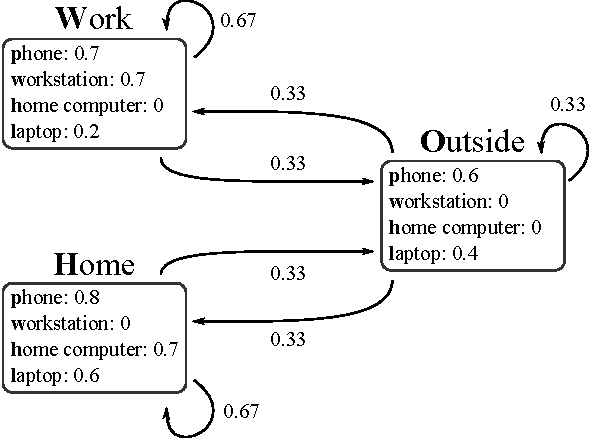
\includegraphics[width=0.9\columnwidth]{figures/hmm.pdf}
\caption{ \label{fig:hmm} Example Hidden Markov Model (HMM) of a user's behavior.}
\end{figure}

HMMs being generative probabilistic models, they allow the generation of observation sequence $O$ given the parameters of the model $\lambda_N$.
Figure~\ref{fig:hmm} shows a possible outcome of the creation of a user's HMM, while figure~\ref{fig:sample_usage} shows an observation sequence $O$ that was generated from the displayed model.

Each round lasts $T=10s$ \commentAL{yes, the user switches places fast} and users start at different times. 
This way, even though the round period is fixed, devices enter and leave the system at different points in the continuous time.


\begin{figure}[t]
\centering
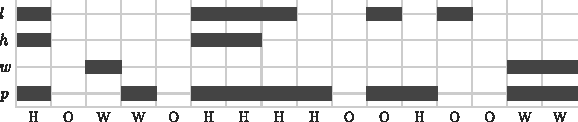
\includegraphics[width=\columnwidth]{figures/sample_usage.pdf}

\caption{\label{fig:sample_usage}Sample device usages using the previous HMM specifications. 
%The bottom line reads the HMM's states: \textbf{W}ork, \textbf{O}utside, and \textbf{H}ome, while the dark lines read when the devices (\textbf{h}ome computer, \textbf{p}hone, and \textbf{w}orkstation) are online.
}
\end{figure}

\subsection{Devices' predictions of the user behavior} % (fold)
\label{sub:devices_predictions_of_the_user_behavior}

% subsection devices_predictions_of_the_user_behavior (end)
\commentAL{Should evaluate the inference of the model given only the observable sequence. Also show that $P[O_{t+1} | S_t] \simeq P[O_{t+i} | S_t]$}

\subsection{Predictive Onion Routes creation} % (fold)
\label{sub:predictive_onion_routes_creation}


In figure \ref{fig:nodes_per_layer_vs_theta} and \ref{fig:success_rate_vs_t}, we computed 10 experiments per set of settings.
$\theta$ is the threshold of the probability that all nodes fail at once: we keep adding nodes to a layer until the layer's probability is below $\theta$. 
It takes the following values: $[0.1, 0.01, 0.001, 0.0001]$.
$L$, the number of layers constituting a route, takes the following values: $[3, 5, 7]$.
The time since route establishment goes from 1 to 10 with  unit step. 
An experiment consisted in $L*5$ users, where we randomly picked pairs of users to compute 20 routes.
Hence, each point in figure~\ref{fig:nodes_per_layer_vs_theta} is the average of 3000 layers size; 
each point in figure~\ref{fig:nodes_per_layer_vs_theta} is the availability rate over 200 routes.

\begin{figure}
\centering
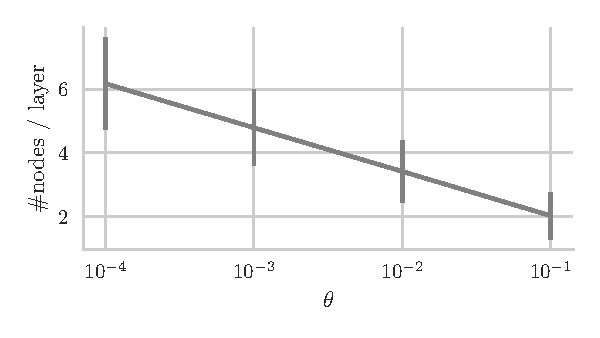
\includegraphics[width=0.8\columnwidth]{figures/nodes_per_layer_vs_theta.pdf}
\caption{\label{fig:nodes_per_layer_vs_theta}Number of nodes per layer of Predictive Onion Route as a function of the parameter $\theta$ (the maximal probability that all nodes in a layer fail at once). We see that the number of nodes exponentially decreases a we relax the $\theta$ constraint.}
\end{figure}

\begin{figure}
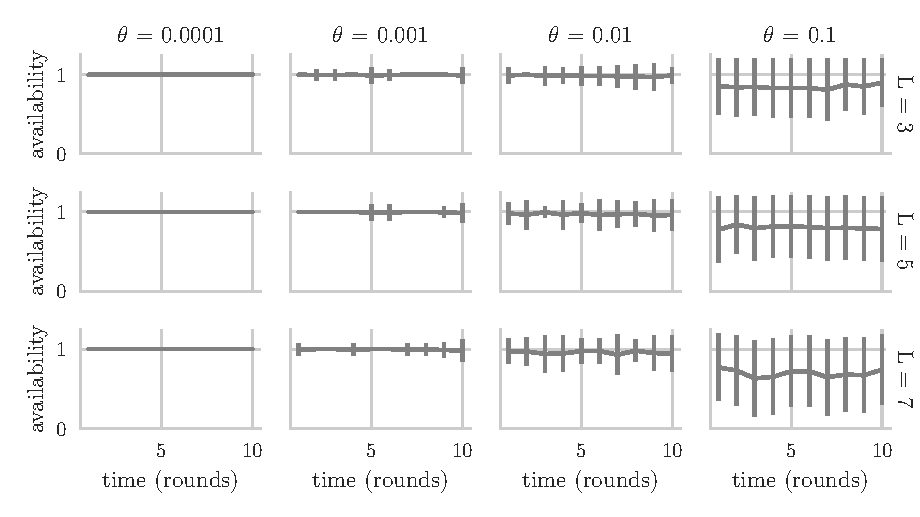
\includegraphics[width=\columnwidth]{figures/success_rate_vs_t.pdf}
\caption{\label{fig:success_rate_vs_t}Availability rate of routes as a function of the time since the route establishment, for several values of the parameters $\theta$ (the maximal probability that all nodes in a layer fail at once) and $L$ (the number of layers in the route).}
\end{figure}
